



% TODO
% sitatatti order kussee.. tässä sitatoidaan meteor b sitatoidaan ekaks ja tässä sitatoidaan mongo i kun senkin pitäisi olla mongo a
% eli kaikki pitää siirtää vähän
% nämä muutokset pitäisi tehdä kun kaikki sitaatit on lisätty missing sitateista
% kappale ennen listaa pitää kirjoittaa uudelleen sillä se on huono
% viimeinen kappale build system pitää suomentaa 




%iso morphic src jos ei käy niin käytä tätä
%https://web.archive.org/web/20221206181248/https://old.gigaom.com/2014/12/27/meteor-wants-to-be-the-warp-drive-for-building-real-time-apps/
% Jonathan Vanian




MeteorJS on avoimeen lähdekoodiin perustuva full-stack JavaScript web-framework, joka on 
suunniteltu nopeaan käyttöönottoon ja kehittämiseen eri laitteille\labciteend{meteor24a}
Meteor mahdollistaa isomorphiseen koodin kirjoittamisen, eli koodiin, joka on samanlaista palvelimella kuten selaimella\labciteend{Kuster23} % en tiedä onko hyvä src mutta on totta joten pitäis löytää jokue
% outo aloittaa taas meteorilla
Meteor ei määritä käytettyä front-end teknologiaa vaan sillä on integraatio moneen yleiseen front-end framework:kiin, kuten Vue, React, Svelte tai Angular\labciteend{meteor24b}{}
Tämä antaa lisä joustoa Meteorille sillä se antaa mahdollisuuden monelle sovelluskehittäjälle, joilla ei ole kokemusta tietystä front-end teknologiasta.\\
\medskip



    

% tukee sana pitää vaihtaa sillä me käytetään sitä itemeissä
Lisäksi Meteor tukee monta ominaisuutta \labcite{meteor24b}:
\begin{itemize}
    \item Tukee monta Front-end kirjastoa ja frameworkkkia
    \item Tukee Typescriptiä
    \item Sisään rakennettu käyttäjä paketti
    \item Toimii monella laitteella
    \item Helppo ja nopea käyttöönottaa 
\end{itemize}
\medskip



Meteorin nopea käyttöönotto on osa johtuen sen paketti järjestelmästä ja valmiiksi paketoiduista paketeista, kuten Meteorin käyttäjät paketti. 
Käyttäjä paketin avusta kehittäjä voi nopeasti luoda todennus (eng authentication) järjestelmän,
joka antaa helpon integraation muiden todennus palvelujen kanssa kuten Facebook, GitHub, Google ym.
Käyttäjä paketti on myös integroitu muihin Meteorin ominaisuuksiin kuten metodeihin.\labcite{meteor24c}



\subsubsection{Meteor metodit}

% toinen kappale
% metodi tekee koodista yksinkertaisemman. metodi tekee rajapinnasta helpomman lukea sillä

% mahdollinen kappale rike kolmannessa kappaleessa


Meteor käyttää Etäkäsittelykutsu (eng Remote procedure call) rajapintaa perinteisen RESTful rajapinnan sijasta\labciteend{meteor24b}
Etäkäsittelykutsussa mallissa asiakasohjelma lähettää palvelinohjelmalle kutsuviestin.
Palvelinohjelma käsittelee kutsuviestin ja suorittaa halutun toiminnon ja palauttaa vastaviestin asiakasohjelmalle.\labcite{ibm23}
Meteorin metodit ominaisuus toimii Etäkäsittelykutsu rajapintana selaimen ja palvelimen välillä. 
\medskip



Meteor metodit ovat palvelimella määriteltyjä funktioita, joita pystytään kutsumaan Meteorin kautta selaimelta tai palvelimelta. 
Kuvassa \nextImageCount{} on esimerkki Meteor metodin määritelmästä.
%selitä yksinkertaisemman eri tavalla, 
Metodit tekevät myös käyttöliittymäkoodista yksinkertaisemman, 
sillä metodien etäkäsittelukutsumalli poistaa käyttöliittymä koodista tarpeen tehdä GET tai POST requesteja palvelimelle.
Metodi funktio käyttää JavaScriptin "this"{} ominaisuutta, jonka
avulla metodiin voidaan antaa kontekstia kutsujasta.
Tässä kontekstissa voi nähdä esimerkiksi onko kutsuja kirjautunut sisään, tai onko kutsujalla oikeat oikeudet kutsua metodia, 
helpottaen turvallisuuden lisäämistä rajapintaan.
\bigskip

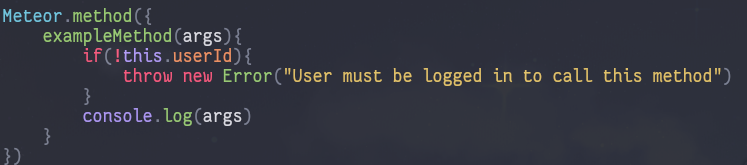
\includegraphics[width=15cm]{src/public/methodexample.png}\\
Kuva \getImgCount {}. Meteor metodin määritelmä
\medskip

Kuvassa on Meteor metodin määritelmä. "exampleMethod"{} metodi katsoo, onko "this"{} ominaisuudessa käyttäjä tunnusta, 
näin metodi voi tietää onko kutsuja kirjautunut sisään,
jos käyttäjä ei ole kirjautunut sisään funktio heittää virheen, joka välitetään kutsujalle.
Jos käyttäjä on kirjautunut sisään, metodi tulostaa argumentit objektin. 
\medskip


%voidaan myös laittaa kuva metodi kutsusta jos halutaan


\subsubsection{Meteor ecosysteemi}

%build system pitää vissii vähä paremmin selittää...
% sdelitetäänkö build system vai.... vaihdetaanko sana johonkin toiseen vaa


Meteor ylläpitää omaa paketointi ekosysteemiään, 
nämä paketit ovat isomorphisia, eli ne toimivat palvelimella ja selaimella\labciteend{pranav17}{}
Meteorilla on ensimmäisen osapuolen paketteja, joita itse Meteor tiimi ylläpitää ja kolmannen osapuolen paketteja,
joita yhteisö ylläpitää. Nämä kolmannen osapuolen paketit voi ladata Meteorin paketti palvelimelle Athmosphere:lle.\labcite{sanders15}
\medskip


Athmosphere on Meteorin ylläpitämä paketti palvelin, johon käyttäjät voivat ladata paketteja tai kirjastoja, jotka ovat suunnattu toimimaan meteorin kanssa.
NPM paketit (eng Node package manager) ovat suunnattu toimimaan NodeJS ympäristössä, ja vaikka ratkaisuja on käyttää NPM paketteja selaimella, 
Athmosphere paketit voi hyöty käyttää Meteorin käännösjärjestelmää (eng build system), jonka avulla paketin kehittäjä voi määritellä mitkä osat ladataan selain puolelle ja mitkä palvelimelle.\labcite{meteor24d}

